%%
%% $Id$
%%
%% Copyright (c) 2007-2008 Christian Fehler
%% Copyright (c) 2007-2008 Benjamin Mies
%%


\chapter{Oberflächengestaltung}\label{GUI}


\section{Redo/Undo}

Da das Lernwerkzeug vom Aussehen her sehr an einen Editor angelehnt ist,
wollten wir dem Benutzer auch eine Möglichkeit geben Schritte rückgängig zu
machen oder wiederherzustellen. Dies war jedoch zu einem Zeitpunkt, zu dem bei
weitem noch nicht alle Funktionalität implementiert war. Desweiteren soll das
Werkzeug ja auch zukünftig an den Stoff der Vorlesung angepasst werden, so dass
uns eine einfache Erweiterbarkeit sehr wichtig war.\vspace{10pt}

Daher haben wir uns entschlossen die Verwaltung der Redo/Undo Schritte nicht
einer Klasse alleine zu überlassen, sondern die verschiedenen Aktionen in
einzelnen Items zu kapseln. Auf diesen Items kann dann die entsprechende redo
bzw. undo Funktion aufgerufen werden. Verwaltet wird dies von einem Handler,
welcher sich nur merkt welches das letzte aktive Item für Redo und Undo ist,
und den Aufruf durch den Nutzer an das Item weiterleitet.\vspace{10pt}

Durch diese Kapselung ist es leicht möglich die Redo/Undo Funktion zu
erweitern, da einfach ein neues Item für die entsprechende Aktion implementiert
werden muss, um diese Item beim Ausführen der Aktion an den Handler zu
übergeben.


\section{Gestaltung der Hauptansicht}

Als wir zu Beginn der Diplomarbeit über die Gestaltung der Hauptansicht
diskutiert haben, kamen wir sehr schnell zu der Übereinkunft, dass die
Ähnlichkeit zu dem Lernwerkzeug TPML möglichst hoch sein sollte. Da sowohl die
Veranstaltung "`Grundlagen der theoretischen Informatik"', als auch "`Theorie
der Programmierung I"' für jeden Informatikstudenten der Universität Siegen
Pflichtveranstaltungen sind, ist die Wahrscheinlichkeit, dass Studenten beide
Lernwerkzeuge nutzen werden sehr hoch.\vspace{10pt}

Ein großer Vorteil von dieser Entscheidung war natürlich, dass wir beide
bereits an der Projektgruppe TPML mitgearbeietet hatten. Zwar waren wir nicht
hauptsächlich für die Grafikelementen beteiligt, konnten aber dennoch einige
Einblicke sammeln, welche uns bei der Grafikgestaltung sehr geholfen
haben.\vspace{10pt}

Unserer Hoffnung ist es, dass zukünftige Benutzer von den parallelen im Aussehen
und in der Funktionsweise beider Lernwerkzeuge profitieren können.\vspace{10pt}

Während der gesamten Diplomarbeit stand im Vordergrund das Lernwerkzeug so
intuitiv und selbsterklärend wie möglich zu gestalten. Denn schließlich soll
ein Benutzer nicht noch lange zeit darauf verwenden müssen, den Umgang mit dem
Werkzeug zu erlernen und sich im schlimmsten Falle durch ein dickes Handbuch
durchzuarbeiten.\vspace{10pt}

Aus diesem Ansatz heraus ist zum Beispiel auch der Wizard zum Anlegen einer
neuen Datei enstanden. Dieser Wizard hat für jedes Eingabefeld ja schon einen
Vorschlag, welche in den Einstellungen auf die Benutzerwünsche angepasst werden
kann. Beim ersten Start sollen diese Werte allerdings als Orientierung und
Beispieldaten dienen, was an diesen Stellen eingetragen werden soll. 


\section{Anpassung aller GUI Komponenten}

Ein wichtiges Konzept bei der graphischen Gestaltung des \gtitool ist es, die von
der Programmiersprache zur Verfügung gestellten Komponenten anzupassen und dann
nur noch ausschließlich diese angepassten Komponenten zu benutzen. Der wohl
größte Vorteil dieser Umsetzung ist, dass nicht überall ein normaler String
verwendet wird, sondern ein sogenannter PrettyString. Dieser enthält neben dem
normalen Text auch noch Farbinformation, sowie Zeichenattribute, wie zum
Beispiel Fettdruck.\vspace{10pt}

Der erforderliche Aufwand wurde investiert, um dem Benutzer eine möglichst
ansprechende Oberfläche zu präsentieren und ihn durch die zusätzlichen
Informationen zu unterstützen, die Inhalte besser zu verstehen.\vspace{10pt}

Ein weiterer wichtiger Ansatz war, dass der Benutzer das \gtitool möglichst
intuitiv bedienen kann. Um dies umzusetzen, wurde unter anderen Drag and Drop
auf den verschiedenen Komponenten implementiert. So kann der Benutzer im
Übergangs-Dialog die Symbole einfach vom "`Alphabet"' in die
"`Übergangs-Menge"' ziehen. Gleiches gilt für das Umsortieren von Produktionen,
das zwar die Grammatik nicht ändert, aber es dem Benutzer ermöglicht die
Produktionen übersichtlicher anzuordnen. In vielen Programmen, in denen Tabs
zur Gliederung benutzt werden, gehört es zum Funktionsumfang diese Tabs per Drag
and Drop zu verschieben. Auch dies wurde implementiert, da es dem Benutzer
erlaubt, seine Daten besser zu organisieren.


\section{Look \& Feel}\label{LookAndFeel}

TODOCF


\section{Zweite Ansicht}\label{SecondView}

Bei der Umsetzung der verschiedenen Algorithmen wurden wir vor das Problem
gestellt, dass es sinnvoll wäre, einen Automaten nach der Umwandlung, mit dem
Automaten oder der Grammatik vor der Umwandlung zu vergleichen. Dies war nur
durch einen Tabwechsel oder das Öffnen eines zweiten \gtitools
möglich.\vspace{10pt}

\begin{figure}[h!]
\begin{center}
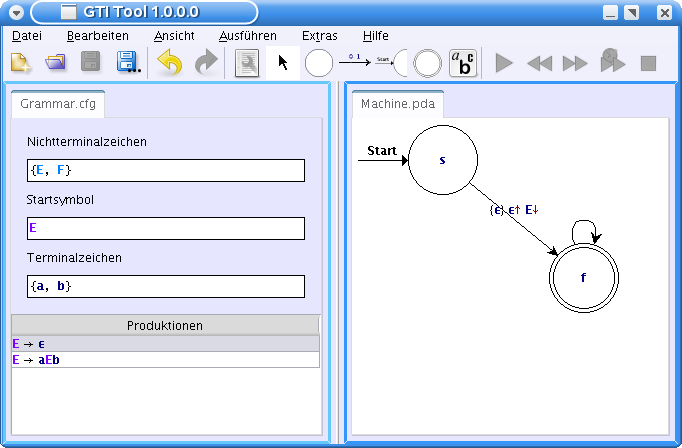
\includegraphics[width=12cm]{../images/second_view.png}
\caption{Zweite Ansicht}
\end{center}
\end{figure}

Das Problem wurde dadurch gelöst, dass eine zweite Ansicht integriert wurde,
die es erlaubt, Tabs in einem zweiten Bereich zu öffnen, so dass zwei Dateien
gleichzeitig sichtbar sind. Während der Umsetzung mussten verschiedene Probleme
diskutiert und gelöst werden. So stellte sich die Frage, wie dem Benutzer
verdeutlicht werden kann, welche der beiden sichtbaren Dateien aktiv ist.
Wichtig ist dieser Status für die Aktivierung der Menüeinträge bzw. Toolbar
Buttons. Als Umsetzung wurde schließlich ausgewählt, dass anhand von
unterschiedlichen Umrandungen dem Benutzer klar gemacht werden soll, welche der
beiden Dateien die aktive ist. Durch dieses Vorgehen wird intuitiv klar, welche
Datei aktiv ist, da sich die Farbe der Umrandung beim Aktivieren der anderen
Ansicht ändert.\vspace{10pt}

Eine weitere wichtige Eigenschaft der zweiten Ansicht ist es, dass Dateien in
diese zweite Ansicht verschoben werden können müssen. Ebenfalls muss es möglich
sein in der zweiten Ansicht Dateien zu öffnen, bzw. neue zu erstellen. Um die
letzen beiden genannten Punkte umzusetzen, wurde das Konzept des aktiven
Editors erweitert. Die oben beschriebene andere Darstellung der aktiven Datei
wurde so erweitert, dass sich auch alle anderen Ereignisse auf den aktiven
Editor beziehen. Wenn eine Datei geöfffnet werden soll, muss erst die Ansicht
aktiviert werden, in der die Datei geöffnet werden soll. Das gleiche gilt beim
Anlegen einer neuen Datei. Das Verschieben von geöffneten Dateien wurde per
Kontextmenü und intuitiv per Drag and Drop zwischen den Ansichten gelöst.
